% !TeX encoding = UTF-8
% !TeX spellcheck = en_US
% !TeX root = ../../Thesis.tex

\chapter{Beam Characterization}
\label{ch:Beam Characterization}

Chapter about beam characterization.

\noindent \textcolor{red}{ignore from here} \\
2020-09-27 set voltages \\
2020-09-30 first successful external run \\
2020-10-07 spot vs pressure \\
2020-10-22 current measurement aluminum foil \\
2020-11-05 forgot to turn off filament heating \\
2020-11-14 assemble chamber with copper rings \\
\textcolor{red}{to here}

\noindent \textbf{possible sections} \\
current and voltage on filament \\
pressure (oxygen exposure) vs beam current \\
aluminum foil \\
What happens with the wobblestick ->  \\
Faraday cup -> Frank \\
Beam current measurement -> Frank \\
Measurement Ablenkungsgeschwindigkeit (frequency) -> Alex \\

\begin{figure}[h]
	\centering
	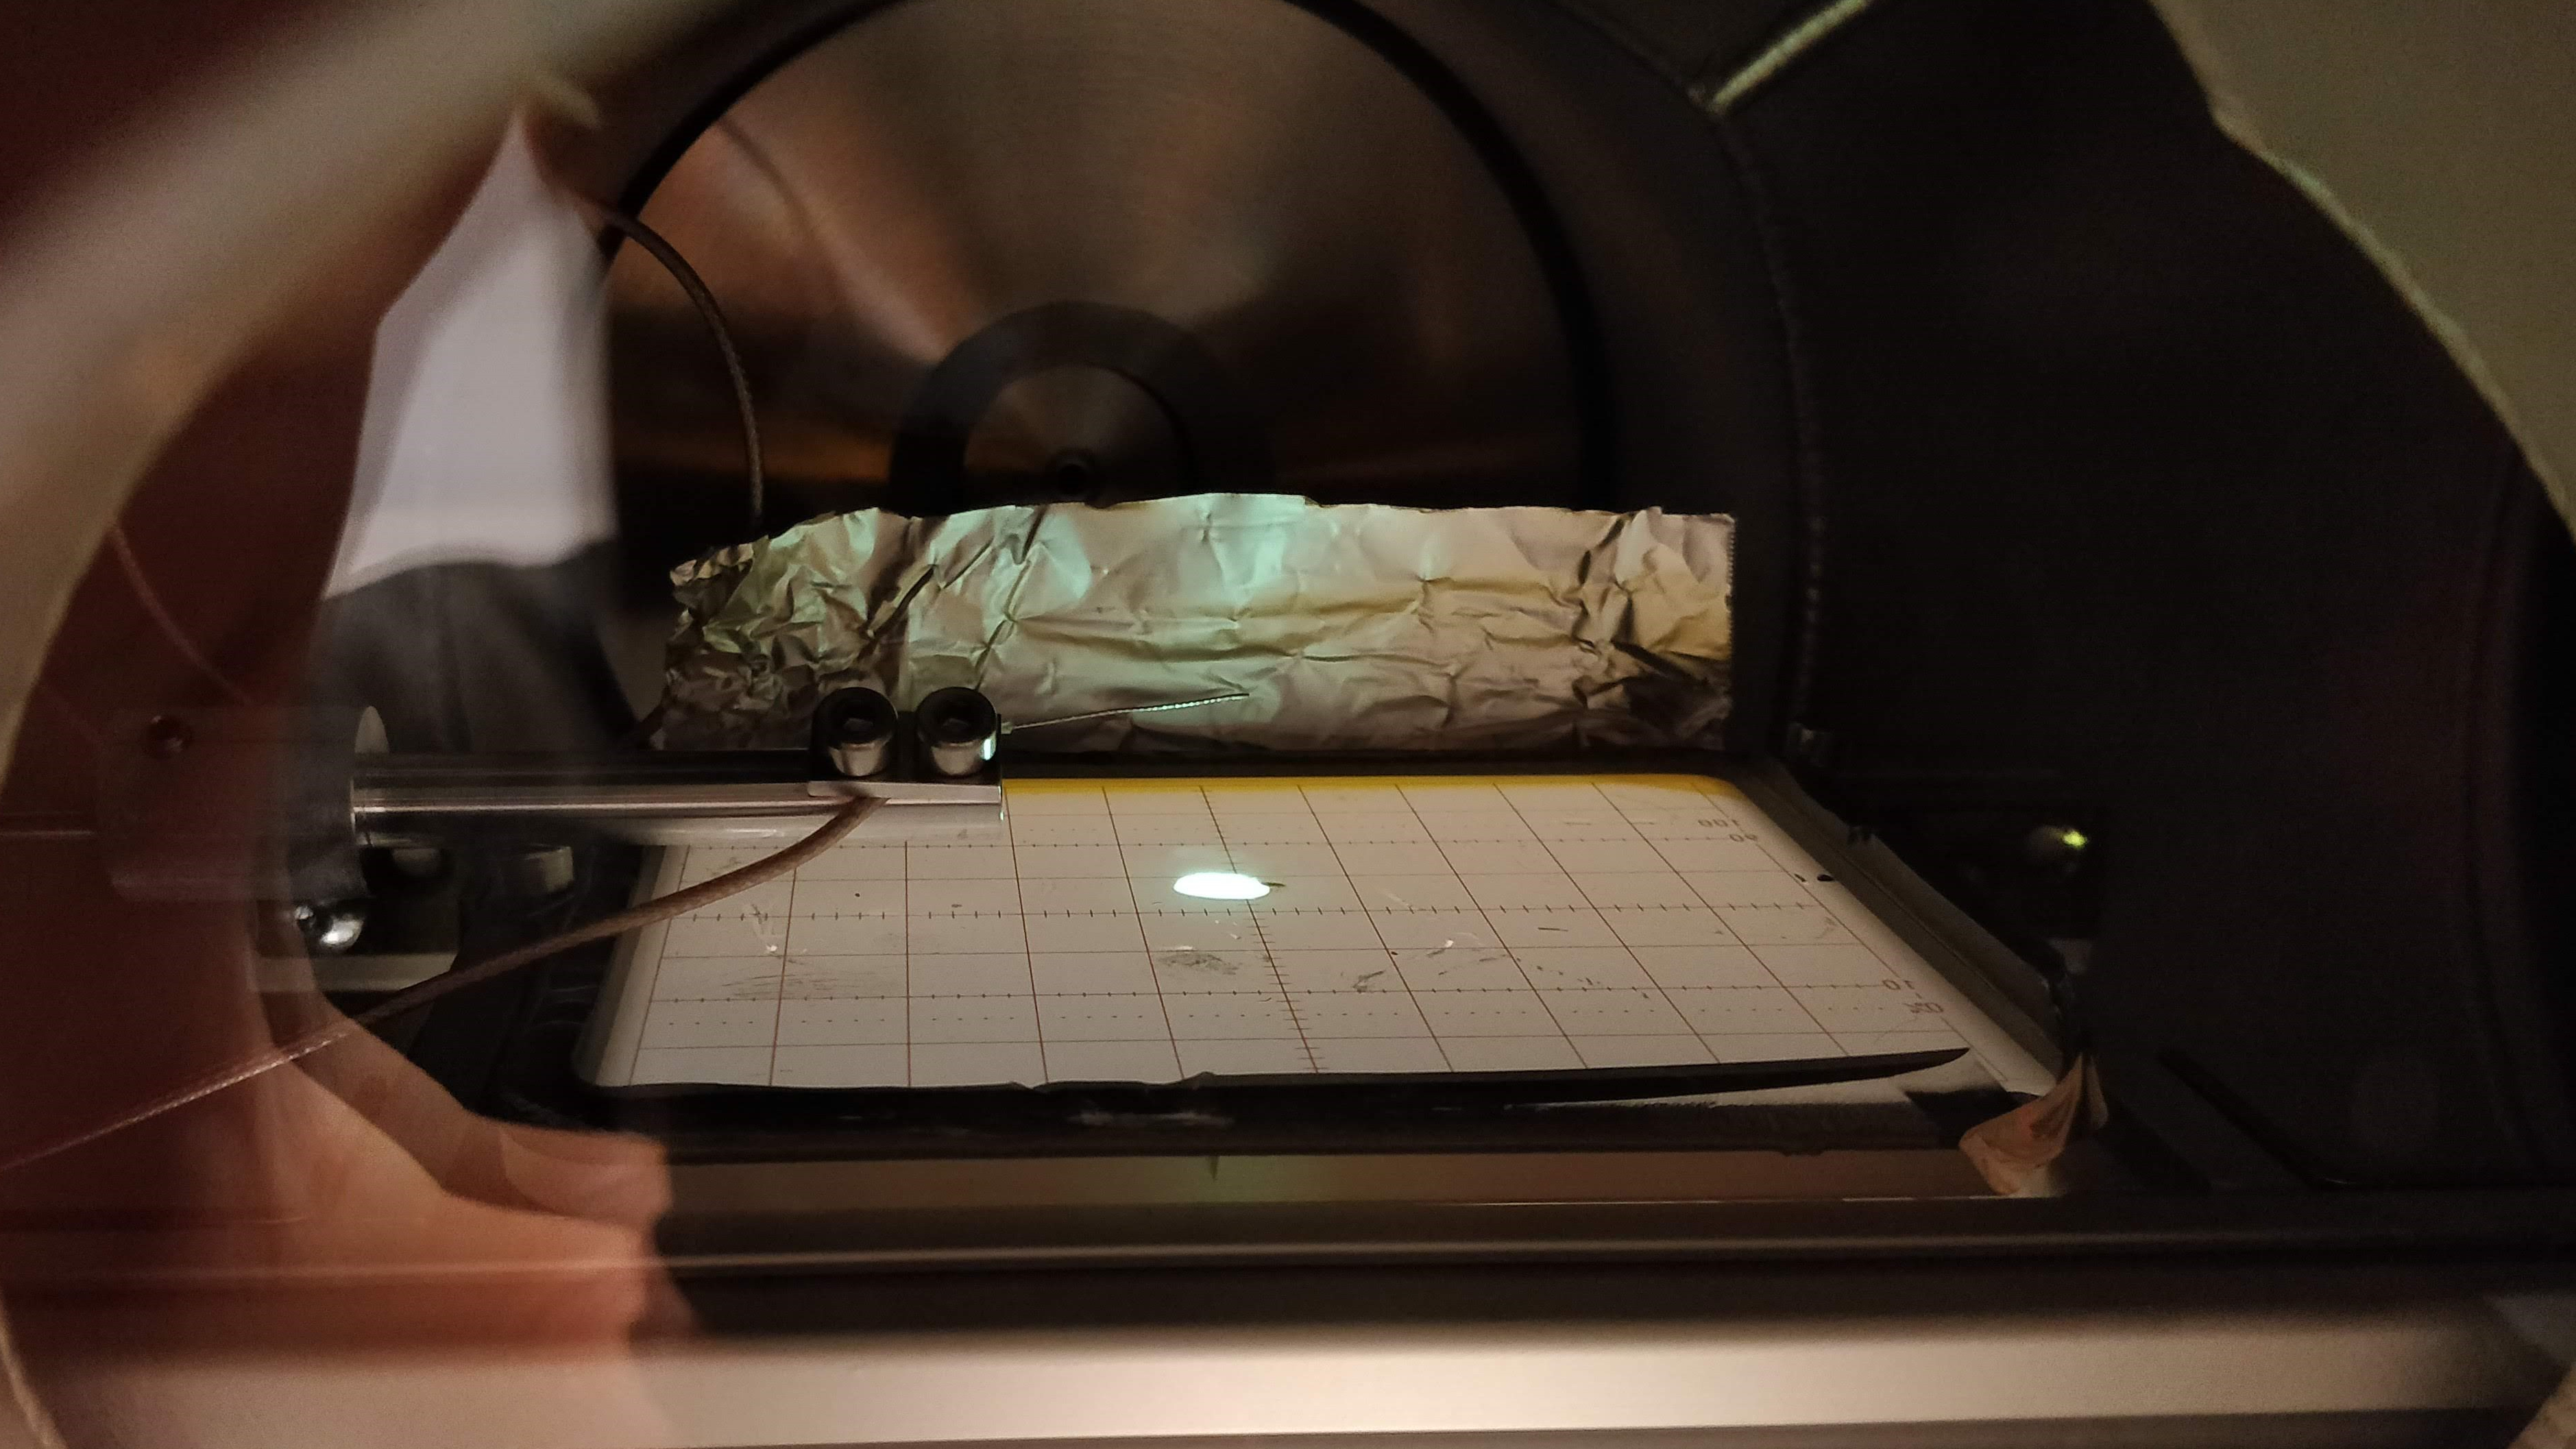
\includegraphics[width=0.9\textwidth]{./Chapters/beam-characterization/center_image}
	\caption{Center image}
	\label{fig:Center image.}
\end{figure}